\documentclass[11pt,a4paper]{article}

\usepackage{geometry}
 \geometry{
 a4paper,
 total={150mm,237mm},
 left=30mm,
 top=30mm,
 }

% cf. http://tex.stackexchange.com/questions/50182/subtitle-with-the-maketitle-page
\usepackage{titling}
\newcommand{\subtitle}[1]{%
  \posttitle{%
    \par\end{center}
    \begin{center}\large\textbf{#1}\end{center}
    \vskip0.5em}%
}

\usepackage{color}
\usepackage{graphicx}
\usepackage[pdftex,colorlinks=false]{hyperref}
% get rid of the horrible coloured boxes around links
\hypersetup{
    colorlinks,%
    citecolor=black,%
    filecolor=black,%
    linkcolor=black,%
    urlcolor=black
}

\usepackage[UKenglish,german]{babel}

\widowpenalty10000  % http://tex.stackexchange.com/questions/4152/how-do-i-prevent-widow-orphan-lines
\clubpenalty10000

\title{The SysSon Platform}
\subtitle{Technical Report TR-2016-08-1\\Institute of Electronic Music and Acoustics, Graz}
\author{Hanns Holger Rutz}
% \date{09-Feb-2016}
\date{August 2016}

% \renewcommand*\rmdefault{dayrom}
% \usepackage{concmath}
\usepackage[lf]{venturis} %% lf option gives lining figures as default; 
			  %% remove option to get oldstyle figures as default
% \renewcommand*\familydefault{\sfdefault} %% Only if the base font of the document is to be sans serif
\usepackage[T1]{fontenc}

% cf. https://tex.stackexchange.com/questions/94126/change-font-to-only-section-and-subsection-of-my-document
%\usepackage{titlesec}
%\titleformat{\chapter}[display]
%  {\fontfamily{pag}\selectfont\huge\bfseries}
%  {\chaptertitlename\ \thechapter}
%  {20pt}
%  {\Huge}
%\titleformat{\section}
%  {\fontfamily{pag}\selectfont\bfseries\Large}
%  {\thesection}
%  {1em}
%  {}
%\titleformat{\subsection}
%  {\fontfamily{pag}\selectfont\bfseries\Large}
%  {\thesection}
%  {1em}
%  {}


\usepackage[utf8]{inputenc}
%\usepackage[backend=biber,natbib=true,citestyle=verbose-ibid,isbn=false,maxnames=3,bibstyle=authoryear,useprefix=true,sorting=ydnt]{biblatex} % citereset=chapter
\usepackage[backend=biber,natbib=true,citestyle=verbose-ibid,isbn=false,maxnames=20,bibstyle=authoryear,firstinits=true,sorting=ydnt,useprefix=true]{biblatex} % citereset=chapter, 
\addbibresource{rutz.bib} % add a bib-reference file

% warning: https://tex.stackexchange.com/questions/313477/
% \usepackage{csquotes}

\usepackage{tabularx}
% cf. https://tex.stackexchange.com/questions/84400/table-layout-with-tabularx-column-widths-502525
\newcolumntype{s}{>{\hsize=1cm}X}

% says you should load after babel and fontspec
\usepackage[shrink=10, babel=true]{microtype}	% http://tex.stackexchange.com/questions/141852/latex-allows-line-break-between-concluding-em-dash-and-comma-before-a-new-sub-cl/141854#141854

\newcommand{\todo}[1]{\colorbox{yellow}{\textsc{todo}: #1}}

\newcommand{\quot}[1]{\guillemotleft {#1}\guillemotright}

\newcommand{\worktitle}[1]{\textit{#1}}

\newcommand{\workentry}[2]{\vspace{7.5pt}\noindent\textbf{#1} (#2)}
\newcommand{\workentrySel}[2]{\vspace{7.5pt}\noindent\textbf{#1}$*$ (#2)}

\newcommand{\figref}[1]{Fig.~\ref{#1}}

\newcommand{\software}[1]{\textit{#1}}

\newcommand{\sysson}[0]{SysSon}
\newcommand{\syssonVersion}[0]{1.8.0}
\newcommand{\syssonVersionS}[0]{1.8.0-SNAPSHOT}

\begin{document}
% \begin{titlepage}
\maketitle
\selectlanguage{UKenglish}
\thispagestyle{empty}
\newpage
\section{\todo{}}

\subsection{Libraries and Modules}

\sysson{} is built with the sbt build tool. Module and library dependencies are managed though Ivy and Maven artifacts, composed of a group-identifier, artifact-identifer, and version. For example, \sysson{} itself has group-id \verb!at.iem.sysson!, artifact-id \verb!sysson!, and current version \verb!1.8.0-SNAPSHOT!. The version scheme is the one proposed as \emph{Semantic Versioning}\footnote{\url{http://semver.org/}}, i.e. \verb!MAJOR.MINOR.PATCH!. The \verb!MAJOR! version indicates an entire new architecture, where the first stable generation is usually indicated by the digit \verb!1!. The \verb!MINOR! version indicates incremental changes, while the \verb!PATCH! version indicate bug fixes without change in functionality.

In the Scala eco-system, the terminology is slightly different, where the major version is called "epoch", the minor version is called major version and the patch version is called minor version. So Scala 2.11.8, the latest release, has epoch 2, major version 11, and minor version 8 in the Scala terminology. We will henceforth use this naming scheme.
The Maven based build tool sbt assumes a \emph{binary compatibility} between all minor versions, whereas the major version must incremented when a binary incompatible change is introduced. A binary incompatibility means that the Java byte code of the library contains change that make it unsafe for use with a caller that was compiled against a different version. This happens for example if a method has been removed from public API or changed in signature. Sbt automatically chooses the highest minor version if there are several transitive dependencies on the same artefact but with different minor versions, while it warns when transitive dependencies exist for the same artefact with different major versions. This also applies to the Scala version a library was compiled against, meaning that a binary file resulting from compilation against Scala 2.10.x (where x is any minor version) is binary incompatible with a binary file resulting from compilation against Scala 2.11.x (with 2.11.8 being the currently most recent release version). To ease this difficulty, sbt has introduced a mechanism called cross-versioning. Often Scala releases are still source compatible, and thus it is possible, for example, to compile the same source code against Scala 2.10.x and 2.11.x without changes. The artefacts will then be "tagged" by appending the major Scala version, e.g. the artifact-id becomes \verb!sysson_2.11! when compiling against Scala 2.11.x (this is independent of the Maven version).

This versioning scheme can be observed in the dependency graph that shows all the libraries and transitive libraries,\footnote{Transitive means a library A is used by another library B, and B is used by \sysson{}. Then A is a transitive dependency of \sysson{}.} generated by the sbt-dependency-graph plugin and shown in \figref{fig:dependencies}.

\begin{figure}%
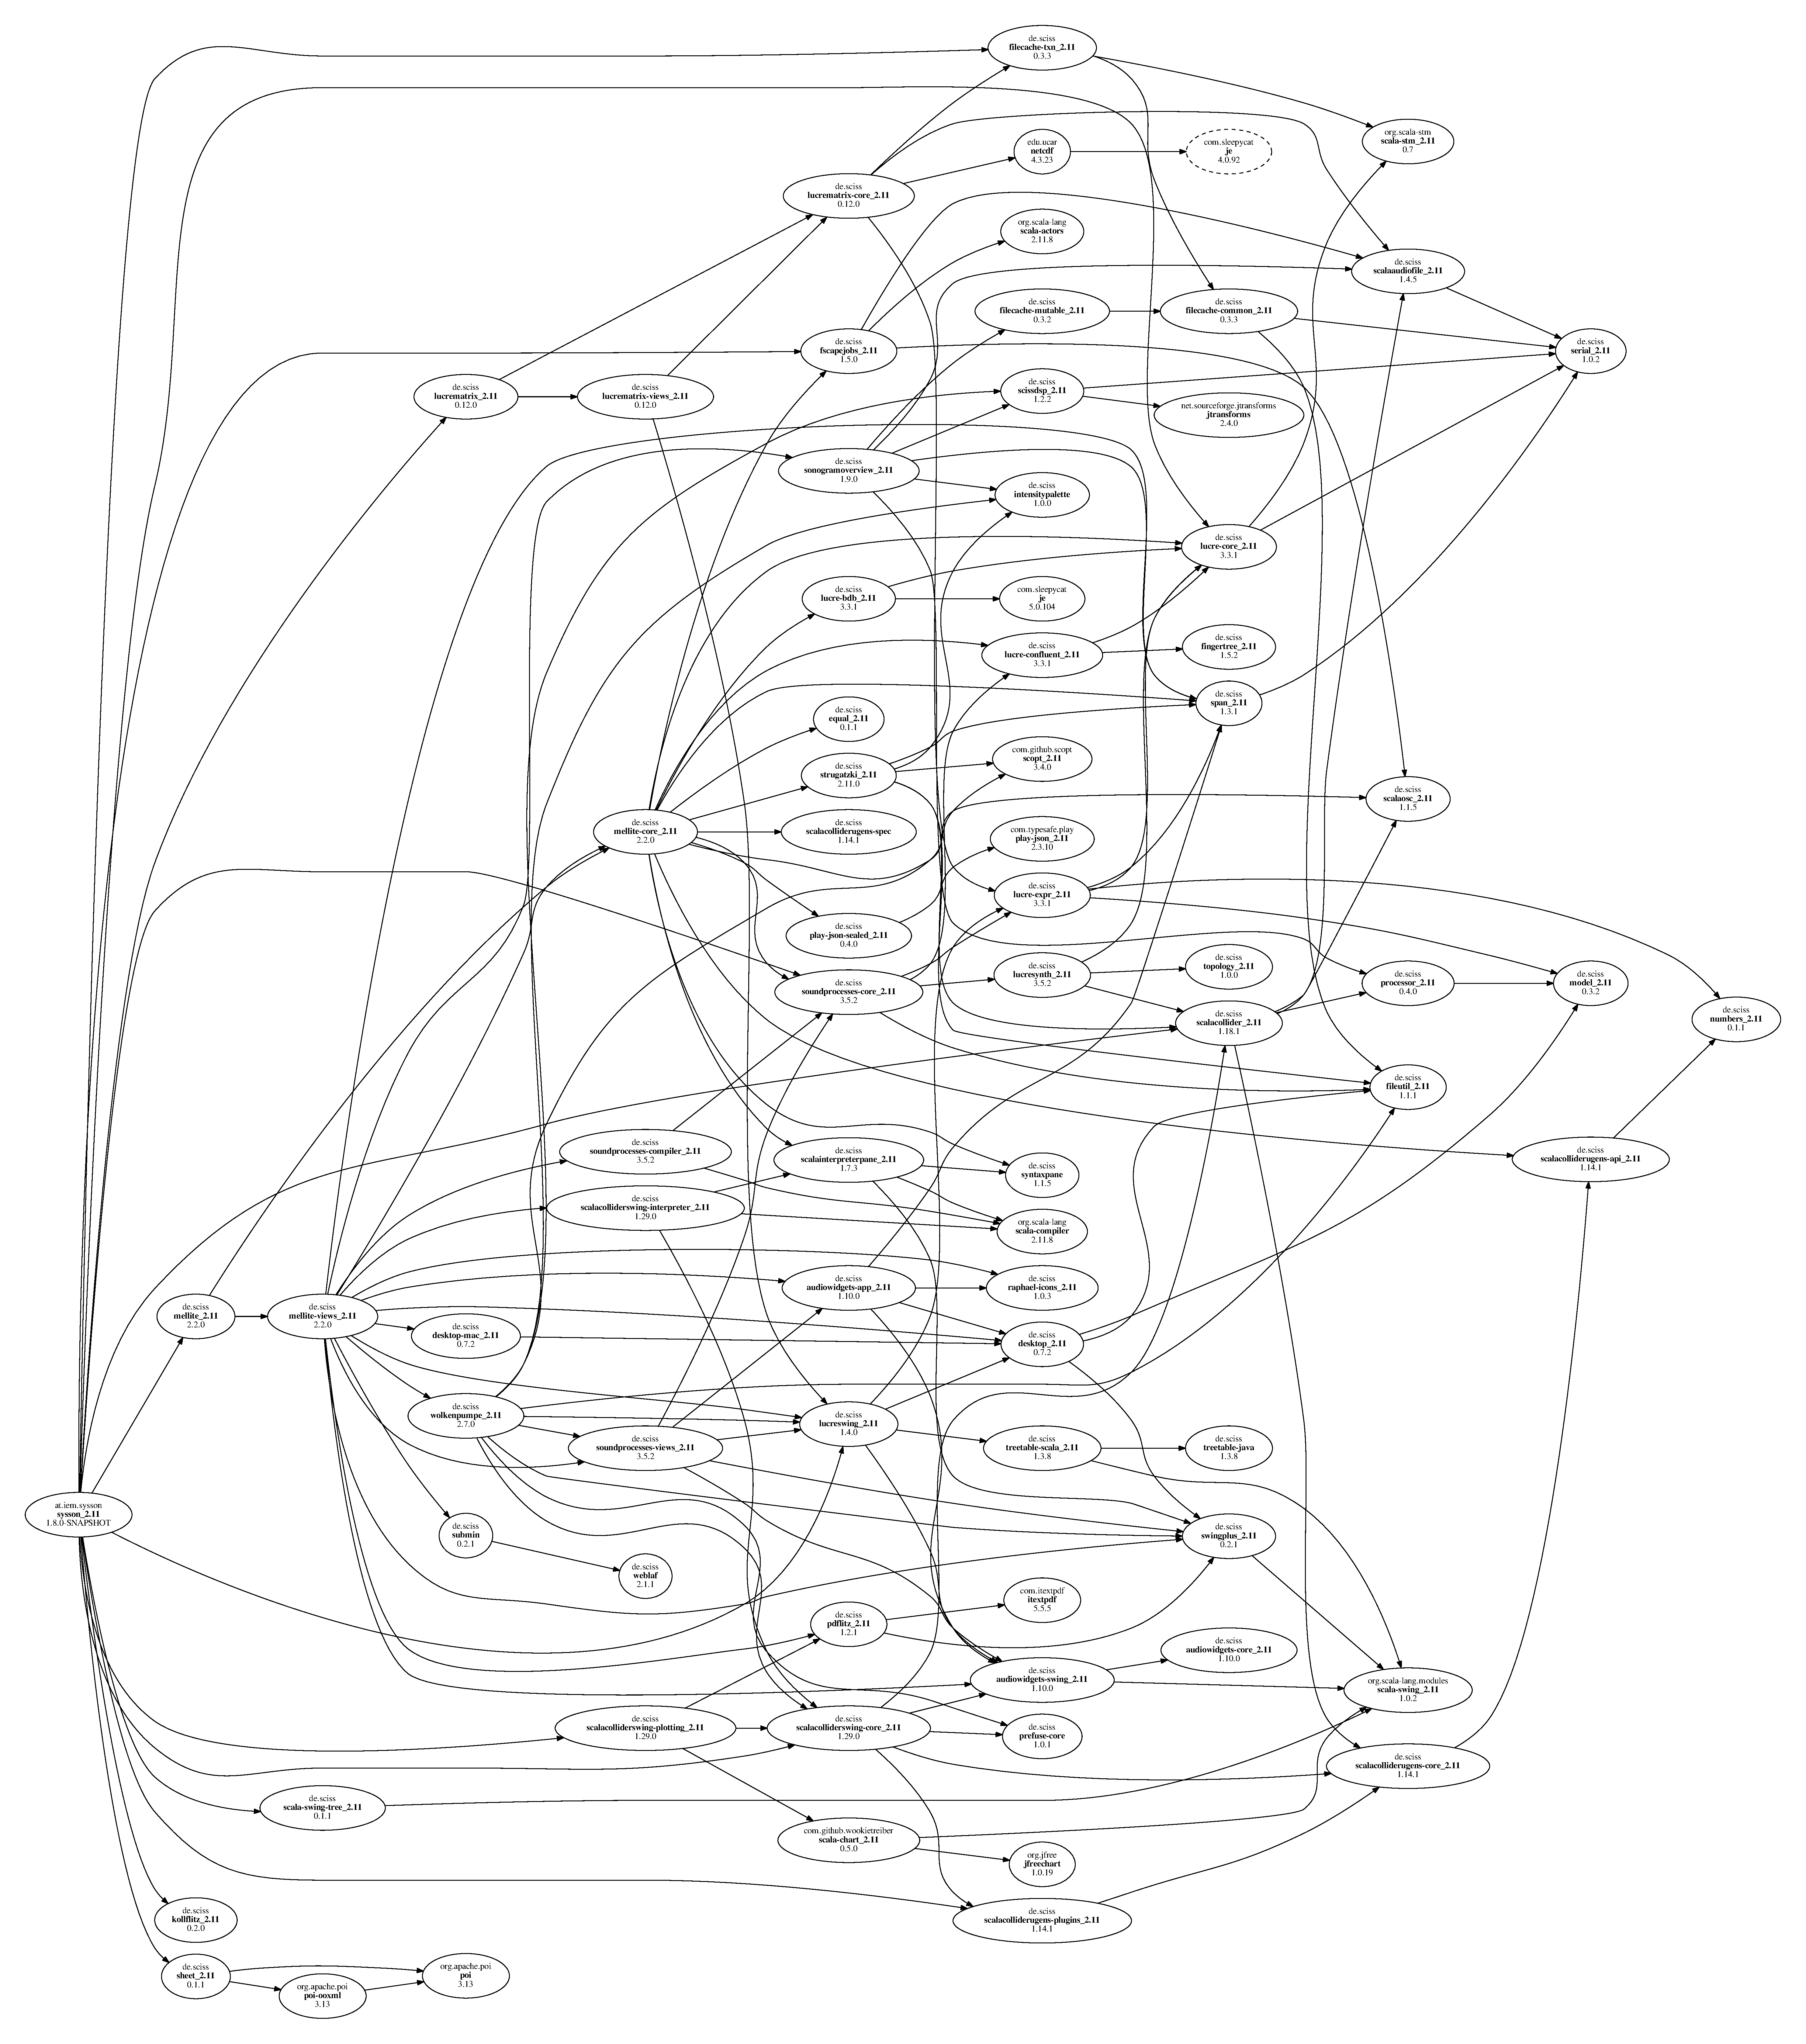
\includegraphics[width=\textwidth,trim=15mm 15mm 15mm 15mm]{figures/dependencies-compile.pdf}%
\caption{Module/library dependencies for SysSon version \syssonVersion{}}%
\label{fig:dependencies}%
\end{figure}

\end{document}
